\documentclass[french]{article}
\usepackage[utf8]{inputenc}
\usepackage[T1]{fontenc}
\usepackage{babel}
\usepackage{lmodern}
\usepackage{graphicx}
\usepackage{tikz}
\usepackage{fullpage}

\usepackage{float}

\usepackage{tabularx}

\usepackage{amsmath}
\usepackage{amsfonts}
\usepackage{amssymb}

\title{Algorithmique 2}
\date{}
\author{L3 RI}

\newcommand{\TODO}{\textcolor{red}{\textbf{TODO}}}

\newcommand{\NP}{\mathrm{NP}}
\newcommand{\size}[1]{\vert #1 \vert}

\begin{document}
\maketitle
\tableofcontents

\section{NP-Complétude}

\subsection{Définitions}

\paragraph{Réduction} Soient $L_1$, $L_2$ des langages.
Une réduction polynomiale de $L_1$ à $L_2$ est une fonction $f$ calculable en temps polynomial telle que :
	\[ f(x) \in L_2 \Longleftrightarrow x \in L_1 \]
On note $L_1 \leq L_2$ ($L_1$ plus facile que $L_2$ = Si on sait résoudre $L_2$, on sait résoudre $L_1$)

\begin{figure}[H]
\center
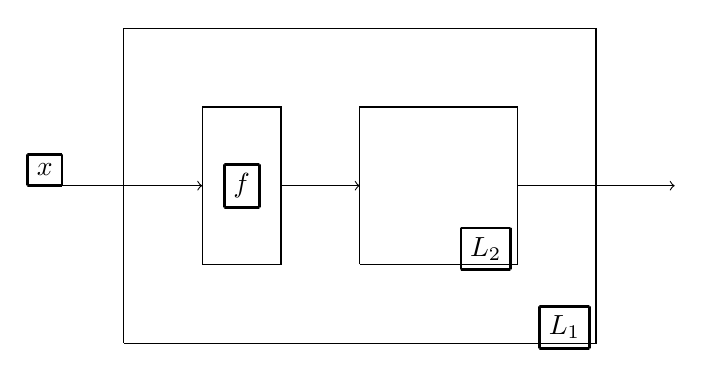
\begin{tikzpicture}
\draw (1,0) -- (1,4) -- (7,4) -- (7,0) -- (1,0);
\draw (2,1) -- (2,3) -- (3,3) -- (3,1) -- (2,1);
\draw (4,1) -- (4,3) -- (6,3) -- (6,1) -- (4,1);
\draw[->] (0,2) -- (2,2);
\draw[->] (3,2) -- (4,2);
\draw[->] (6,2) -- (8,2);
\node[draw,line width=-1] at (0,2.2) {$x$};
\node[draw,line width=-1] at (2.5,2) {$f$};
\node[draw,line width=-1] at (5.6,1.2) {$L_2$};
\node[draw,line width=-1] at (6.6,0.2) {$L_1$};
\end{tikzpicture}
\caption{Schéma de réduction de $L_1$ à $L_2$}
\end{figure}

\paragraph{Classe NP}Soit $L$ un langage. $L$ est dit dans la classe NP s'il existe une machine de Turing non-déterministe en temps polynomial par rapport à la taille de l'entrée qui décide $L$.

\paragraph{NP-Complétude} Soit $L$ un langage. $L$ est dit NP-dur si pour tout $L' \in \NP$, $L' \leq L$.
$L$ est dit NP-complet si $L \in \NP$ et $L$ est NP-dur.

\paragraph{Remarques} Si un problème NP-complet est dans P, alors P = NP. Pour montrer que $L'$ est NP-dur, il suffit de montrer qu'il existe $L$ NP-dur tel que $L \leq L'$.

\subsection{Satisfiabilité d'une formule}

\vspace{0.5cm}
\begin{tabularx}{\textwidth}{p{1cm}X}
\multicolumn{2}{c}{\textbf{Problème de décision : SAT}} \\ 
\emph{Entrée} & $\varphi$ formule de la logique propositionnelle \\ 
\emph{Sortie} & Oui si $\varphi$ est satisfiable, c'est-à-dire s'il existe une valuation $v$ des variables qui rend $\varphi$ vraie \\
\end{tabularx}

\paragraph{Théorème de Cook} SAT est NP-complet. (\emph{Réduction de $L$ à SAT pour $L \in \NP$ en considérant une machine de Turing $\mathcal{M}$ non-déterministe qui décide $L$. On construit une formule qui traduit une exécution de $\mathcal{M}$.})

\vspace{0.5cm}
\begin{tabularx}{\textwidth}{X}
\multicolumn{1}{c}{\textbf{Problème de décision : $i$-SAT}} \\ 
Restriction de SAT à des formules en forme normale conjonctive (CNF) tel que chaque clause contient au plus $i$ littéraux \\
\end{tabularx}

\paragraph{Théorème} 3-SAT est NP-complet. (\emph{Réduction de SAT à 3-SAT.})

\paragraph{Théorème} 2-SAT est dans P. (\emph{Réduction de 2-SAT à la détermination des CFC d'un graphe.})

\vspace{0.5cm}
\begin{tabularx}{\textwidth}{p{1cm}X}
\multicolumn{2}{c}{\textbf{Problème de décision : MAX-2-SAT}} \\ 
\emph{Entrée} & $\varphi$ formule en 2-forme normale conjonctive et $k \in \mathbb{N}$ \\ 
\emph{Sortie} & Oui s'il existe une valuation qui satisfait au moins $k$ clauses de $\varphi$ \\
\end{tabularx}

\paragraph{Théorème} MAX-2-SAT est NP-complet. (\emph{Réduction de 3-SAT à MAX-2-SAT.})

\subsection{Graphes}

\vspace{0.5cm}
\begin{tabularx}{\textwidth}{p{1cm}X}
\multicolumn{2}{c}{\textbf{Problème de décision : ENS\_INDEP}} \\ 
\emph{Entrée} & $G = (V, E)$ un graphe non-orienté et $k \in \mathbb{N}$ \\ 
\emph{Sortie} & Oui s'il existe $V' \subseteq V$ tel que $\size{V'} = k$ et $(V' \times V') \cap E = \varnothing$ \\
\end{tabularx}

\paragraph{Théorème} ENS\_INDEP est NP-complet. (\emph{Réduction de 3-SAT à ENS\_INDEP.})


\vspace{0.5cm}
\begin{tabularx}{\textwidth}{p{1cm}X}
\multicolumn{2}{c}{\textbf{Problème de décision : MAX\_CUT}} \\ 
\emph{Entrée} & $G = (V, E)$ un graphe non-orienté et $k \in \mathbb{N}$ \\ 
\emph{Sortie} & Oui s'il existe $S_1$ et $S_2$, $S = S_1 \uplus S_2$ et $\# \lbrace (u,v) \in E ~\vert~ u \in S_1 \text{ et } v \in S_2 \rbrace \geq k$ \\
\end{tabularx}

\paragraph{Théorème} MAX\_CUT est NP-complet. (\emph{Réduction de MAX-2-SAT à MAX\_CUT}.)

\section{Algorithmes d'approximation}

\TODO

\section{Algorithmes probabilistes}

\TODO

\section{Géométrie algorithmique}

\subsection{Enveloppe convexe}

\vspace{0.5cm}
\begin{tabularx}{\textwidth}{p{1cm}X}
\multicolumn{2}{c}{\textbf{Calcul de l'enveloppe convexe}} \\ 
\emph{Entrée} & Un ensemble $S$ de points $(x,y)$ du plan \\ 
\emph{Sortie} & $C \subseteq S$ une énumération dans le sens trigonométrique des points extrémaux de l'enveloppe convexe de S \\
\end{tabularx}

\paragraph{Position d'un point par rapport à une droite} On suppose qu'il n'existe pas trois points alignés. $p_2$ est à gauche de la droite orientée $(\vec{p_0p_1})$ si et seulement si :
 \[ \det(\vec{p_0p_1}, \vec{p_0p_2}) > 0 \]
 
\paragraph{Marche de Jarvis} Algorithme du paquet cadeau
\begin{itemize}
	\item Partir du point de plus petite ordonnée $p_0$
	\item Prendre un point suivant, parcourir tous les points et le remplacer s'il en existe un plus à gauche de la droite orientée $(\vec{p_{actuel}~p_{suivant}})$
	\item Recommencer jusqu'à retomber sur $p_0$
\end{itemize}

\paragraph{Complexité de la marche de Jarvis} Si $n$ est la taille de $S$ et $h$ le nombre de points dans l'enveloppe convexe : $O(nh)$

La complexité dépend de la sortie (\emph{output sensitive}).


\paragraph{Balayage de Graham}\TODO

\paragraph{Complexité du balayage de Graham}\TODO

\subsection{Points les plus rapprochés}

\vspace{0.5cm}
\begin{tabularx}{\textwidth}{p{1cm}X}
\multicolumn{2}{c}{\textbf{Points les plus rapprochés}} \\ 
\emph{Entrée} & Un ensemble $S$ de points $(x,y)$ du plan \\ 
\emph{Sortie} & $d^*$ la distance minimale entre deux points de $S$ \\
\end{tabularx}

\paragraph{Algorithme}Principe de diviser pour régner, on divise le plan en deux. On obtient récursivement $\delta_D$ et $\delta_G$. Soit $\delta = \min (\delta_G, \delta_D)$. On considère l'ensemble $M$ des points dans la bande de largeur $2\delta$. $M = p_1 \ldots p_k$ énumérés par ordonnées croissantes.

\paragraph{Lemme}S'il existe $i < j$ tel que $d(p_i,p_j) < \delta$ alors il existe $i' < j' \leq i'+8$ tel que $d(p_{i'},p_{j'}) < \delta$.

En effet, on considère un rectangle qu'on divise en huit parties. On peut alors prendre 9 points et appliquer le principe des tiroirs.

\paragraph{Complexité} Pré-tris en $O(n \log n)$. Au total, avec le \emph{Master Theorem} : $O(n \log n)$

\section{Algorithmes distribués}





\end{document}
